\ylDisplay{Läätsed} % Ülesande nimi
{Tundmatu autor} % Autor
{lõppvoor} % Voor
{2013} % Aasta
{P 7} % Ülesande nr.
{3} % Raskustase
{
% Teema: Valgusõpetus
\ifStatement
Jukul on suur hulk nõgusläätsi, mille fookuskauguste leidmiseks ta konstrueeris lihtsa
süsteemi. Ta suunas optilise peateljega paralleelse laserikiire läbimõõduga $2R$ tuntud
fookuskaugusega $f_1$ koondava läätse keskpunkti, pärast mida koondus laserkiir ühte punkti
ekraanil. Kui nüüd panna fookuskaugusega $f_2$ nõguslääts võrdsele kaugusele koondavast
läätsest ja ekraanist, on laserkiire läbimõõt ekraanil $2r$. Leidke $f_2$ eeldusel, et $2f_2 < f_1$.
\begin{center}
	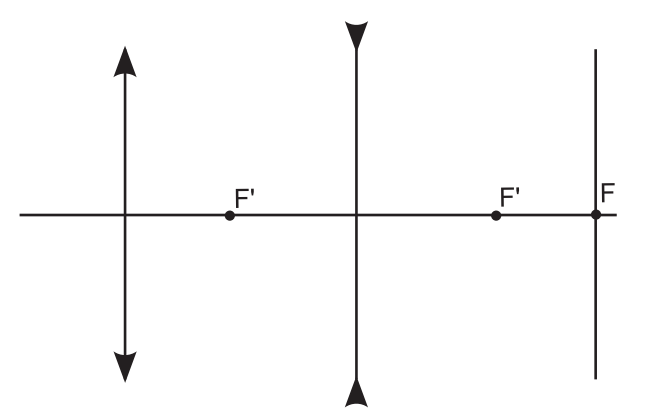
\includegraphics[width=0.5\linewidth]{2013-v3p-07-yl.png}
\end{center}
\fi
\ifHint
Kogu pilt on optilise peatelje suhtes sümmeetriline, tänu millele võib tegeleda ainult ühe poolega. Konstrueeri kiirte käik, teades et kõigi nõgusläätse läbivate paralleelsete kiirte pikendused lõikuvad fokaaltasandil.
\fi
\ifSolution
Kogu pilt on optilise peatelje suhtes sümmeetriline, tänu sellele  saame tegeleda ainult ühe poolega. Konstrueerime kiirte käigu, teades et kõigi nõgusläätse läbivate paralleelsete kiirte pikendused lõikuvad fokaaltasandil.
Joonisel on mõned meid huvitavad sarnased kolmnurgad $\triangle AF^\prime D \sim \triangle BO ^\prime D \sim \triangle CF ^\prime D$ ja $\triangle EOF \sim \triangle AF ^\prime O \sim BO ^\prime F$. Lisaks teame osade lõikude pikkusi: $\mid EO \mid = R$, $\mid OF \mid f_1$, $\mid F ^\prime O ^\prime \mid = f_2$ ja $\mid CF \mid = r$. Seda teades saab moodustada neljast võrrandist koosneva lineaarvõrrandisüsteemi.
\\
Lahendus 1 \\
\[
\cfrac{\mid EO \mid}{\mid OF \mid} = \cfrac{\mid AF^\prime \mid}{F ^\prime O} 
\]
\[
\cfrac{\mid EO \mid}{\mid OF \mid} = \cfrac{\mid BO ^\prime \mid}{O ^\prime F}
\]
\[
\cfrac{\mid AF^\prime \mid}{\mid F^\prime D \mid} = \cfrac{\mid CF \mid}{\mid FD \mid}
\]
\[
\cfrac{\mid AF^\prime \mid}{\mid F^\prime D \mid} = \cfrac{\mid B^\prime O \mid}{O^\prime D} 
\]
\[
\cfrac{R}{f_1} = \cfrac{\mid AF^\prime \mid}{f_2} 
\]
\[
\cfrac{R}{f_1} = \cfrac{\mid BO ^\prime \mid}{\frac{f_1}{2}}
\]
\[
\cfrac{\mid AF^\prime \mid}{\mid O^\prime D \mid - f_2} = \cfrac{r}{\frac{f_1}{2} + \mid O ^\prime D \mid}
\]
\[
\cfrac{\mid AF^\prime \mid}{\mid O ^\prime D \mid - f_2} = \cfrac{\mid B^\prime O \mid}{O^\prime D} 
\]
\\
\begin{center}
	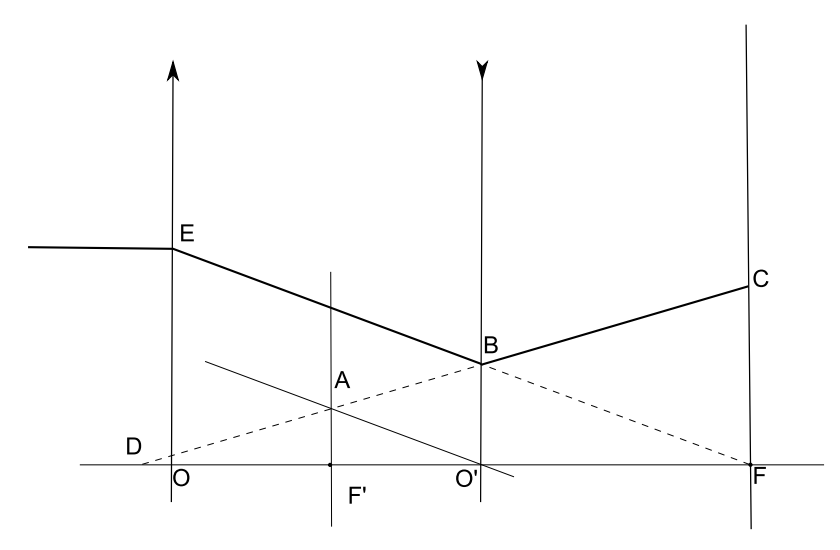
\includegraphics[width=0.5\linewidth]{2013-v3p-07-lah1.png}
\end{center}
Pärast süsteemi lahendamist saame tulemuseks 
\begin{center}
$f_2 = \cfrac{R}{4r} f_1$.
\end{center}

Lahendus 2 \\
Selles lahenduses kasutame läätse valemit $- \frac{1}{f} = \frac{1}{a} - \frac{1}{k}$. $f$ ees on miinus kuna tegemist on nõgusläätsega ja $k$ ees on miinus kuna tegemist on näiva kujutisega. Kasutades kiirte pööratavuse printsiipi vaatame hoopis olukorda, kus tekib objektist $CF$ näiv kujutis $AB$. Lisaks kasutame kolmnurkade sarnasust: $\triangle CFO ^\prime \sim \triangle ABO ^\prime$ ja $\triangle DOF \sim \triangle ABF$.

\[
\cfrac{\mid CF \mid}{\mid FO ^\prime \mid} = \cfrac{\mid AB \mid}{BO ^\prime}
\]
\[
\cfrac{\mid DO \mid}{\mid OF \mid} = \cfrac{\mid AB \mid}{\mid BF \mid}
\]
\[
- \cfrac{1}{f_2} = \cfrac{1}{\mid F O ^\prime \mid} - \cfrac{1}{\mid BO ^\prime\mid}
\]
\[
\cfrac{r}{\frac{f_1}{2}} = \cfrac{\mid AB \mid}{\mid BO ^\prime \mid}
\]
\[
\cfrac{R}{f_1} = \cfrac{\mid AB \mid}{\frac{f_1}{2} - \mid BO^\prime \mid}
\]
\[
- \cfrac{1}{f_2} = \cfrac{1}{\frac{f_1}{2}} - \cfrac{1}{\mid BO ^\prime \mid}
\]
\begin{center}
	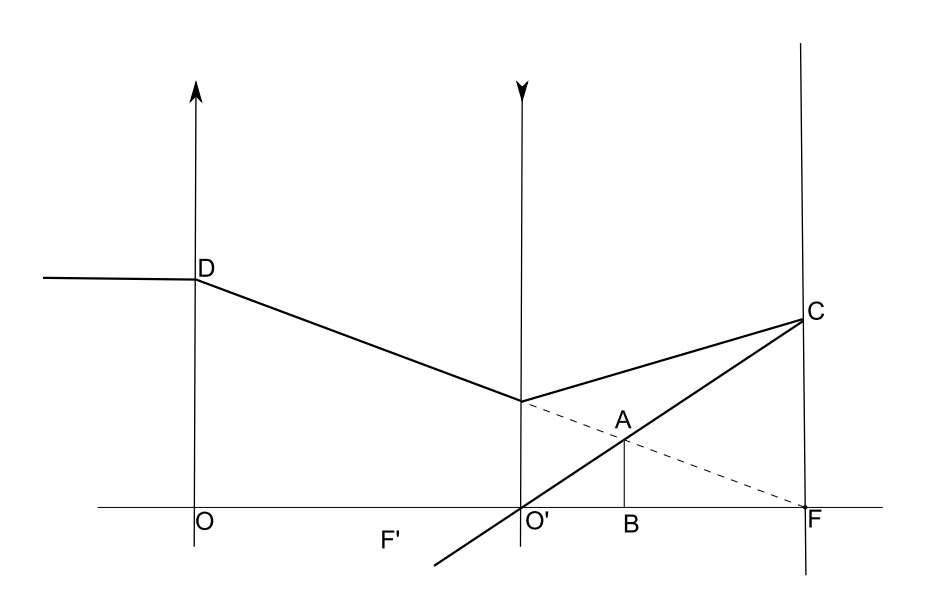
\includegraphics[width=0.5\linewidth]{2013-v3p-07-lah2.png}
\end{center}
Selle võrrandisüsteemi lahendamisel saame $f_2 = \cfrac{R}{4r}f_1$.
\fi
}